\documentclass[mathserif,10pt]{beamer}

\usepackage{beamerthemesplit}
\usepackage{graphics}
\usepackage{epsfig}
\usepackage{algorithm}
\usepackage{verbatim}
\usepackage{listings}
\usepackage{framed}
\usepackage{pstricks}
\usepackage{pst-node,pst-tree}
\usepackage{pst-rel-points}
\usepackage{flexiprogram}
\usepackage[UKenglish]{babel}
\usepackage{hyperref}
\usepackage{pst-coil}
\usepackage{color}
\usepackage{epsfig}
%\usepackage{tikz}
%\usepackage{multirow}

\usefonttheme{serif}

\newcommand{\cmt}[1]{}
%\noindent

\setcounter{tocdepth}{1}


\usepackage{color}
 
\definecolor{codegreen}{rgb}{0,0.6,0}
\definecolor{codegray}{rgb}{0.5,0.5,0.5}
\definecolor{codepurple}{rgb}{0.58,0,0.82}
\definecolor{backcolour}{rgb}{0.95,0.95,0.92}
\lstdefinestyle{mystyle}{
    %backgroundcolor=\color{backcolour},   
    commentstyle=\color{codegreen},
    keywordstyle=\color{magenta},
    %numberstyle=\tiny\color{codegray},
    stringstyle=\color{codepurple},
    basicstyle=\footnotesize,
    breakatwhitespace=false,         
    breaklines=true,                 
    captionpos=b,                    
    keepspaces=true,                 
    %numbers=left,                    
    %numbersep=5pt,                  
    showspaces=false,                
    showstringspaces=false,
    showtabs=false,                  
    tabsize=2
}
 
\lstset{style=mystyle,frameround=fttt}


\setbeamercovered{transparent=0}

  \usetheme{CambridgeUS}
  \usecolortheme{dolphin}

  \title[GRI]{GRI: \textbf{I}nterpreter of a dynamic language for \textbf{GR}aph algorithms}
  \author[]{{\textbf{Sandeep Dasgupta}} }
  \begin{document}

  \begin{frame}
  \titlepage
  \end{frame}
  \usebeamertemplate{mytheme}

  \AtBeginSection[]
{
  \begin{frame}<beamer>
    \frametitle{Outline}
  \tableofcontents[currentsection]
    \end{frame}
}

\defverbatim[colored]\lstdfs{
\begin{lstlisting}[language=C++,basicstyle=\tiny,keywordstyle=\color{red}]
  define("NUM_VERTICES", "10");
  define("NOTVISITED", "0");
  define("VISITED", "1");

  function dfs(v)
  {
      if(v.visit == VISITED)
        return;

      println("Closing vertex: " + v.num);
      v.visit = VISITED;

      foreach(neighbor; v.getNeighbors())
        dfs(neighbor);
  }

  function main(argv)
  {
    g = graph();
    g.loadFromFile(argv[0]);

    dfs(first);
  }

\end{lstlisting}
}

\section{Motivation}
\frame
{
  \frametitle{\secname}
  \begin{itemize}[<+->]
    \item Graphical models are applied to widely varying fields.
    \begin{itemize}
      \item Biochemistry 
        \cmt{genomics}
      \item Electrical Engineering
        \cmt{communication networks }
      \item Computer Science
        \cmt{Algorithms and computation}
      \item Operations Research
        \cmt{Scheduling}
      \item Organizational Structures 
        \cmt{social networking}
    \end{itemize} 
    \vspace{1cm}
    \item Field experts often struggle to represent \& allow computations on  graphical models in \textbf{Convenient} and \textbf{Efficient} way.
      \cmt{
Convenience: is essential so that even for domain experts who are not coding experts
can code and reason about their implementation. Ease of interface could be due to:
– Expressive power of the language representing those models.
– Intuitive extensibility of the language.
– Ability of the language to provide exploratory programming, where the user may
experiment with different ideas (without dwelling much into the language syntax)
before coming to a conclusive one.

Designed language need to be efficient in the following sense.
– Underlying design decisions including data structures need to be carefully crafted to
achieve expected run-time w.r.t the input size.
– Implementation need to be scalable w.r.t the space/time requirements. This is im-
portant because most of the graph algorithm typically work on huge input sizes.

To meet all above goals and most importantly exploratory programming, we decided to work
on a dynamically typed language to represent graphs and apply various computations on them.
With a dynamically typed language the user do not have to worry much about declaring types
and can focus mostly on his/her experiments.
      }
    \vspace{1cm}
  \end{itemize} 
}

\section{Language}
\subsection{Syntax \& Semantics}
\frame
{
  \begin{figure}[h]
  \centering
  \scalebox{0.80}{
    \includegraphics{Figs/1.eps}
  }
  \end{figure}
}
\frame
{
  \begin{figure}[h]
  \centering
  \scalebox{0.80}{
    \includegraphics{Figs/2.eps}
  }
  \end{figure}
}
\frame
{
  \begin{figure}[h]
  \centering
  \scalebox{0.70}{
    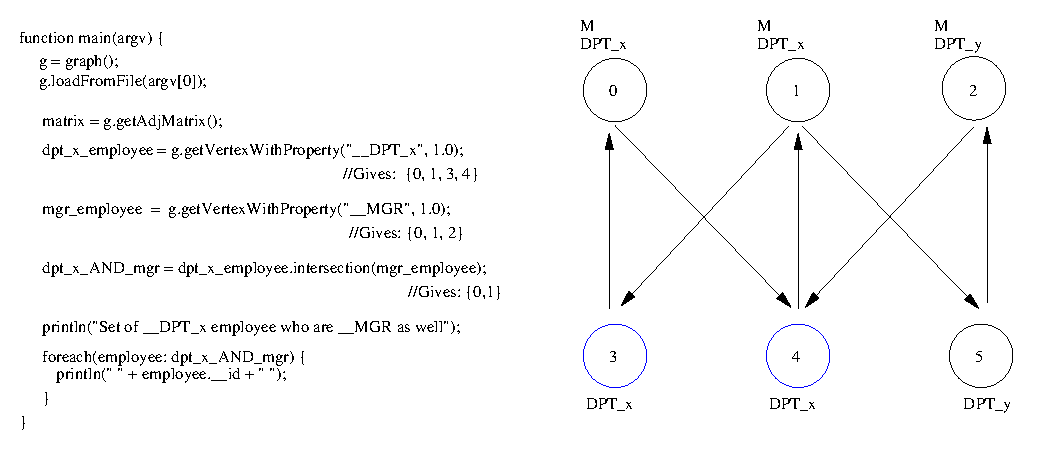
\includegraphics{Figs/3.eps}
  }
  \end{figure}
}
\frame
{
  \begin{figure}[h]
  \centering
  \scalebox{0.73}{
    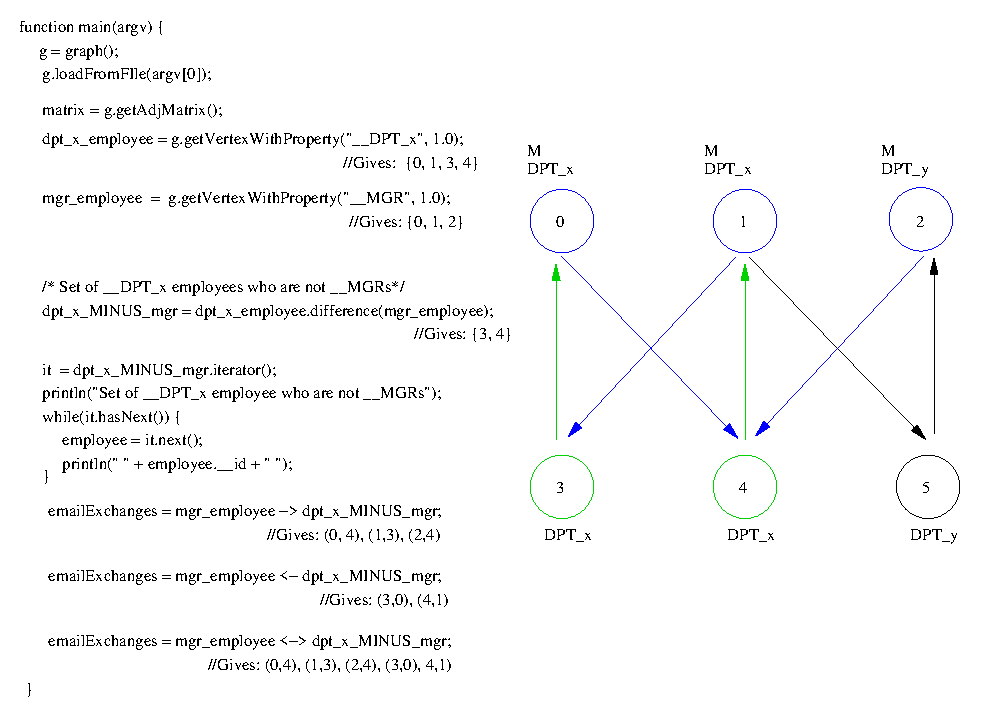
\includegraphics{Figs/4.eps}
  }
  \end{figure}
}

\frame
{
  \frametitle{\subsecname}
  \lstdfs
}

\section{Questions?}
\subsection{Questions?}
\frame
{}

\end{document}
